% MH1812 — Chapter 8: Number Theory (0->100 ground-up)
\chapter[Number Theory]{Number Theory: Divisibility, GCD, Modular Arithmetic and RSA Intuition}
\label{ch:numbertheory}

\begin{quote}
\emph{``God made the integers, all else is the work of man.''} --- Leopold Kronecker. Integers under division and remainders hide the mathematics behind cryptography.
\end{quote}

\noindent\fbox{\parbox{\dimexpr\linewidth-2\fboxsep-2\fboxrule}{%
\textbf{From zero: sharing and remainders.} Start with ``$a$ divides $b$'' as exact sharing, build the division algorithm (quotient + remainder), compute greatest common divisors (Euclid), work on clocks (modular arithmetic), and glimpse how RSA turns these ideas into secrecy.}}
\vspace{0.4em}

\section*{Learning Outcomes}
After this chapter you will be able to:
\begin{enumerate}[label=(L\arabic*)]
    \item define divisibility, prime, composite, and apply the division algorithm;
    \item compute $\gcd$ and $\mathrm{lcm}$ via Euclid and prime factorisation;
    \item solve linear congruences and compute modular inverses when they exist;
    \item state and apply Fermat's little theorem and Chinese remainder intuition;
    \item explain RSA key generation, encryption and decryption at a high level.
\end{enumerate}

% ============================================================
\section{Divisibility and the Division Algorithm}
\label{sec:divisibility}
For $a,b\in\mathbb{Z}$, $a\mid b$ (``$a$ divides $b$'') if $\exists k\in\mathbb{Z}\,b=ak$. Then $a$ is a divisor, $b$ a multiple. Every $n\neq0$ divides $0$; $a\mid b\land b\mid a\Rightarrow |a|=|b|$.

\begin{theorem}[Division algorithm]
For $a\in\mathbb{Z}$, $d\in\mathbb{Z}^+$ there exist unique $q,r$ with $a=dq+r$ and $0\le r<d$. $q$ is quotient, $r=a\bmod d$ remainder.
\end{theorem}
\begin{proof} Existence by well-ordering on $\{a-dk\ge0\}$; uniqueness by gap $<d$.
\end{proof}

A \emph{prime} $p\ge2$ has divisors $1,p$ only; \emph{composite} otherwise. $1$ is neither. Fundamental theorem (proved via Euclid's lemma): every $n\ge2$ factors uniquely into primes.

\begin{figure}[h]\centering
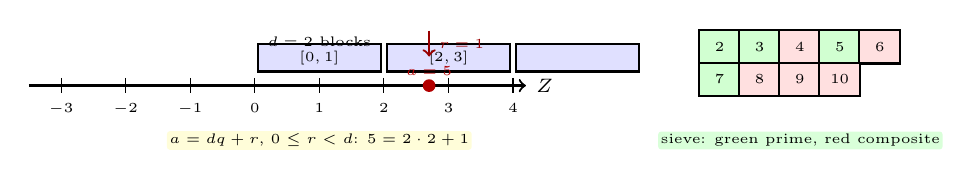
\begin{tikzpicture}[scale=0.82,every node/.style={font=\scriptsize}]
% Number line division algorithm visualisation
\draw[->,thick] (-3.5,0)--(4.2,0) node[right] {$\mathbb{Z}$};
\foreach \x in {-3,-2,-1,0,1,2,3,4} {\draw (\x,0.12)--(\x,-0.12) node[below,font=\tiny] {$\x$}; }
\foreach \x in {0,1,2} {\draw[thick,fill=blue!12] (\x*2+0.05,0.22) rectangle++(1.9,0.42);}
\node[font=\tiny] at (1.0,0.68) {$d=2$ blocks};
\node[font=\tiny] at (1.0,0.43) {$[0,1]$};
\node[font=\tiny] at (3.0,0.43) {$[2,3]$};
\fill[red!70!black] (2.7,0) circle (2.8pt) node[above,font=\tiny] {$a=5$};
\draw[thick,red!60!black,->] (2.7,0.85)--(2.7,0.45) node[midway,right,font=\tiny] {$r=1$};
\node[font=\tiny,fill=yellow!15,rounded corners=1pt,inner sep=1pt] at (1.0,-0.85) {$a=dq+r$, $0\le r<d$: $5=2\cdot2+1$};
% Prime sieve table
\begin{scope}[xshift=7.2cm,yshift=0.6cm]
\foreach \i/\n in {0/2,1/3,2/4,3/5,4/6,5/7,6/8,7/9,8/10} {
  \pgfmathsetmacro{\x}{mod(\i,5)*0.62}
  \pgfmathsetmacro{\y}{-int(\i/5)*0.5}
  \pgfmathparse{\n==2||\n==3||\n==5||\n==7 ? "green!18" : "red!12"}
  \edef\col{\pgfmathresult}
  \node[draw,thick,fill=\col,minimum width=0.52cm,minimum height=0.42cm,font=\tiny] at (\x,\y) {$\n$};
}
\node[font=\tiny,fill=green!15,rounded corners=1pt,inner sep=1pt] at (1.25,-1.45) {sieve: green prime, red composite};
\end{scope}
\end{tikzpicture}
\caption{Division algorithm partitions $\mathbb{Z}$ into blocks of length $d$; remainder $r$ is offset inside the block.}
\label{fig:division-alg}
\end{figure}

\begin{lemma}[Divisibility lemmas]
If $a\mid b$ and $a\mid c$ then $a\mid(bx+cy)$ for any $x,y\in\mathbb{Z}$ (linear combination). If $a\mid b$ and $b\neq0$ then $|a|\le|b|$.
\end{lemma}

\section{GCD and Euclid}
\label{sec:gcd}
$\gcd(a,b)$ is the greatest $d$ with $d\mid a$ and $d\mid b$; $\mathrm{lcm}(a,b)$ the least positive common multiple. $\gcd(0,b)=|b|$; $\gcd(a,b)=\gcd(b,a\bmod b)$.

Euclid's algorithm iterates $(a,b)\mapsto(b,a\bmod b)$ until $b=0$; variant strictly decreases, $\gcd$ invariant, $O(\log\min(a,b))$ steps because remainder $<a/2$ when $b\le a$.

\begin{figure}[h]\centering
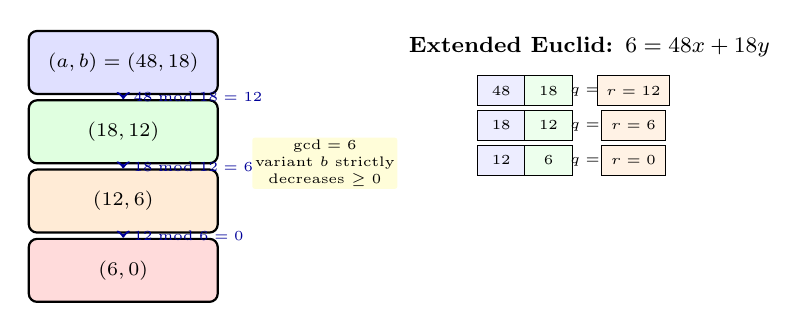
\begin{tikzpicture}[scale=0.80,every node/.style={font=\scriptsize}]
% Euclid steps visualisation
\node[draw,thick,rounded corners=3pt,fill=blue!12,minimum width=2.4cm,minimum height=0.8cm] (s0) at (0,1.8) {$(a,b)=(48,18)$};
\node[draw,thick,rounded corners=3pt,fill=green!12,minimum width=2.4cm,minimum height=0.8cm] (s1) at (0,0.7) {$(18,12)$};
\node[draw,thick,rounded corners=3pt,fill=orange!16,minimum width=2.4cm,minimum height=0.8cm] (s2) at (0,-0.4) {$(12,6)$};
\node[draw,thick,rounded corners=3pt,fill=red!14,minimum width=2.4cm,minimum height=0.8cm] (s3) at (0,-1.5) {$(6,0)$};
\draw[->,thick,blue!60!black] (s0)--(s1) node[midway,right,font=\tiny] {$48\bmod18=12$};
\draw[->,thick,blue!60!black] (s1)--(s2) node[midway,right,font=\tiny] {$18\bmod12=6$};
\draw[->,thick,blue!60!black] (s2)--(s3) node[midway,right,font=\tiny] {$12\bmod6=0$};
\node[font=\tiny,fill=yellow!15,rounded corners=1pt,inner sep=1pt,align=center] at (3.2,0.2) {$\gcd=6$\\variant $b$ strictly\\decreases $\ge0$};
% Extended Euclid table
\begin{scope}[xshift=6.0cm,yshift=0.7cm]
\node[font=\footnotesize\bfseries] at (1.4,1.35) {Extended Euclid: $6=48x+18y$};
\foreach \i/\a/\b/\q/\r in {0/48/18/2/12,1/18/12/1/6,2/12/6/2/0} {
  \pgfmathsetmacro{\y}{0.65-\i*0.55}
  \node[font=\tiny,draw,fill=blue!7,minimum width=0.6cm,minimum height=0.38cm] at (0,\y) {$\a$};
  \node[font=\tiny,draw,fill=green!7,minimum width=0.6cm,minimum height=0.38cm] at (0.75,\y) {$\b$};
  \node[font=\tiny,minimum width=0.5cm] at (1.45,\y) {$q=\q$};
  \node[font=\tiny,draw,fill=orange!10,minimum width=0.6cm,minimum height=0.38cm] at (2.1,\y) {$r=\r$};
}
\end{scope}
\end{tikzpicture}
\caption{Euclid's algorithm: repeated remainder steps; extended version finds $x,y$ with $ax+by=\gcd(a,b)$.}
\label{fig:euclid}
\end{figure}

\begin{theorem}[B\'ezout]
$\gcd(a,b)$ is the smallest positive linear combination $ax+by$. Hence $a,b$ coprime ($\gcd=1$) iff $\exists x,y\,ax+by=1$.
\end{theorem}

Extended Euclid finds such $x,y$ by back-substitution; crucial for modular inverses.

\begin{lstlisting}[language=Python]
def egcd(a,b):
    if b==0: return (a,1,0)
    g,x1,y1=egcd(b, a % b)
    return (g, y1, x1 - (a//b)*y1)

print(egcd(48,18))  # (6, -1, 3) => -1*48 + 3*18 = 6
def inv_mod(a,m):
    g,x,y=egcd(a,m)
    assert g==1, "no inverse"
    return x % m
print(inv_mod(3,11))  # 4 because 3*4=12=1 mod 11
\end{lstlisting}

\section{Modular Arithmetic}
\label{sec:modular}
$a\equiv b\pmod m$ iff $m\mid(a-b)$ iff $a\bmod m=b\bmod m$. Residues $\mathbb{Z}_m=\{0,\dots,m-1\}$ form a clock.

\begin{figure}[h]\centering
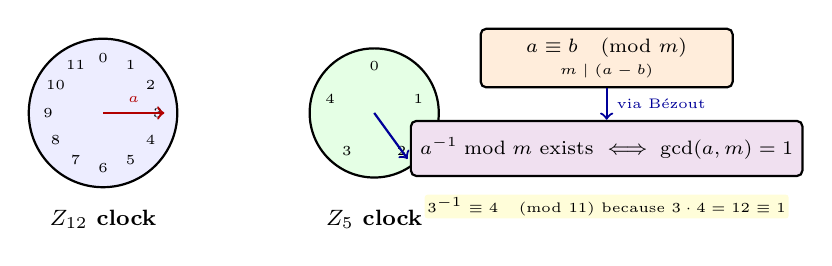
\begin{tikzpicture}[scale=0.82,every node/.style={font=\scriptsize}]
% Clock mod 12 and mod 5
\begin{scope}
\draw[thick,fill=blue!7] (0,0) circle (1.15);
\foreach \i in {0,...,11} {\pgfmathsetmacro{\ang}{90-\i*30} \node[font=\tiny] at (\ang:0.85) {$\i$};}
\draw[->,thick,red!70!black] (0,0)--(90-3*30:0.95) node[midway,above,font=\tiny] {$a$};
\node[font=\footnotesize\bfseries] at (0,-1.65) {$\mathbb{Z}_{12}$ clock};
\end{scope}
\begin{scope}[xshift=4.2cm]
\draw[thick,fill=green!10] (0,0) circle (1.0);
\foreach \i in {0,...,4} {\pgfmathsetmacro{\ang}{90-\i*72} \node[font=\tiny] at (\ang:0.72) {$\i$};}
\draw[->,thick,blue!60!black] (0,0)--(90-2*72:0.88);
\node[font=\footnotesize\bfseries] at (0,-1.65) {$\mathbb{Z}_5$ clock};
\end{scope}
\begin{scope}[xshift=7.8cm]
\node[draw,thick,fill=orange!14,rounded corners=2pt,minimum width=3.2cm,minimum height=0.7cm,align=center] (c1) at (0,0.85) {$a\equiv b\pmod m$\\{\tiny $m\mid(a-b)$}};
\node[draw,thick,fill=violet!12,rounded corners=2pt,minimum width=3.2cm,minimum height=0.7cm,align=center] (c2) at (0,-0.55) {$a^{-1}\bmod m$ exists $\iff\gcd(a,m)=1$};
\draw[->,thick,blue!60!black] (c1)--(c2) node[midway,right,font=\tiny] {via B\'ezout};
\node[font=\tiny,fill=yellow!15,rounded corners=1pt,inner sep=1pt] at (0,-1.45) {$3^{-1}\equiv4\pmod{11}$ because $3\cdot4=12\equiv1$};
\end{scope}
\end{tikzpicture}
\caption{Modular arithmetic as clock arithmetic. Invertibility depends on coprimality.}
\label{fig:mod-clock}
\end{figure}

Arithmetic mod $m$: $(a+b)\bmod m$, $(a\cdot b)\bmod m$ stay in $\mathbb{Z}_m$. Division by $a$ means multiply by $a^{-1}\bmod m$, which exists iff $\gcd(a,m)=1$.

\begin{theorem}[Fermat's little theorem]
If $p$ prime and $p\nmid a$ then $a^{p-1}\equiv1\pmod p$, hence $a^p\equiv a\pmod p$ always.
\end{theorem}
\begin{proof}[Sketch] Non-zero residues permuted by multiplication by $a$; product $1\cdot2\cdots(p-1)\equiv a^{p-1}\cdot1\cdot2\cdots(p-1)$.
\end{proof}

Chinese remainder theorem (CRT): for coprime $m_1,m_2$, the pair $(a\bmod m_1,a\bmod m_2)$ uniquely determines $a\bmod m_1m_2$; it stitches clocks together.

\section{RSA Intuition}
\label{sec:rsa}
RSA turns Fermat/Euler into a trapdoor. Pick large primes $p,q$, $n=pq$, $\phi(n)=(p-1)(q-1)$. Choose $e$ coprime to $\phi(n)$ (public exponent), compute $d\equiv e^{-1}\pmod{\phi(n)}$ (private, via extended Euclid). Public key $(n,e)$, private $d$.

Encrypt $m\in[0,n)$: $c=m^e\bmod n$. Decrypt: $m=c^d\bmod n$ because $m^{ed}=m^{1+k\phi(n)}\equiv m$ by Euler ($a^{\phi(n)}\equiv1$ when coprime; CRT handles rest).

Security rests on hardness of factoring $n$ to get $\phi(n)$; correctness on modular inverse and FLT/Euler.

\begin{lstlisting}[language=Python]
# Toy RSA (tiny primes -- never use like this in production!)
p, q = 61, 53
n = p*q; phi = (p-1)*(q-1)
e = 17
# d = e^{-1} mod phi
def egcd(a,b):
    if b==0: return (a,1,0)
    g,x1,y1=egcd(b,a%b)
    return (g,y1,x1-(a//b)*y1)
d = egcd(e,phi)[1] % phi
m = 42
c = pow(m,e,n)
m2 = pow(c,d,n)
print(f"n={n} phi={phi} e={e} d={d} c={c} decrypted={m2}")
assert m==m2
\end{lstlisting}

\begin{remark}[Why not just $m^e$?]
Modular exponentiation via repeated squaring keeps numbers $<n^2$; $m^e$ without mod would be astronomically huge ($\approx2^{2048}$ bits for real RSA-2048).
\end{remark}


\begin{theorem}[Euler's theorem]
If $\gcd(a,m)=1$ then $a^{\phi(m)}\equiv1\pmod m$, where $\phi$ is Euler's totient. FLT is the prime case $\phi(p)=p-1$.
\end{theorem}

\begin{example}[Modular exponentiation]
$2^{10}\bmod1000$ computed by squaring: $2^2=4,2^4=16,2^8=256,2^{10}=256\cdot4=1024\equiv24$; no need for huge intermediates.
\end{example}

Divisibility is the discrete analogue of inequality: $a\mid b$ means $b$ is a multiple of $a$.
Division algorithm is Euclidean division: every integer sits uniquely in a block of size $d$ with remainder $r$.
Primes are the atoms of multiplication, uniquely factoring every integer beyond $1$.
Euclid's algorithm is the oldest non-trivial algorithm, its logarithmic steps still optimal.
B\'ezout's identity shows $\gcd(a,b)$ is not just a divisor but a linear combination, enabling inverses.
Modular arithmetic is clock arithmetic: numbers wrap around after $m$, forming the ring $\mathbb{Z}_m$.
Invertible residues mod $m$ are exactly those coprime to $m$, counted by Euler's totient $\phi(m)$.
Fermat's little theorem gives a fast exponent reduction, powering primality tests and RSA.
Chinese remainder theorem stitches independent clocks into one, enabling parallel modular computations.
RSA's security rests on factoring being hard while multiplying primes is easy, a computational asymmetry.
Divisibility is the discrete analogue of inequality: $a\mid b$ means $b$ is a multiple of $a$.
Division algorithm is Euclidean division: every integer sits uniquely in a block of size $d$ with remainder $r$.
Primes are the atoms of multiplication, uniquely factoring every integer beyond $1$.
Euclid's algorithm is the oldest non-trivial algorithm, its logarithmic steps still optimal.
B\'ezout's identity shows $\gcd(a,b)$ is not just a divisor but a linear combination, enabling inverses.
Modular arithmetic is clock arithmetic: numbers wrap around after $m$, forming the ring $\mathbb{Z}_m$.
Invertible residues mod $m$ are exactly those coprime to $m$, counted by Euler's totient $\phi(m)$.
Fermat's little theorem gives a fast exponent reduction, powering primality tests and RSA.
Chinese remainder theorem stitches independent clocks into one, enabling parallel modular computations.
RSA's security rests on factoring being hard while multiplying primes is easy, a computational asymmetry.
Divisibility is the discrete analogue of inequality: $a\mid b$ means $b$ is a multiple of $a$.
Division algorithm is Euclidean division: every integer sits uniquely in a block of size $d$ with remainder $r$.
Primes are the atoms of multiplication, uniquely factoring every integer beyond $1$.
Euclid's algorithm is the oldest non-trivial algorithm, its logarithmic steps still optimal.
B\'ezout's identity shows $\gcd(a,b)$ is not just a divisor but a linear combination, enabling inverses.
Modular arithmetic is clock arithmetic: numbers wrap around after $m$, forming the ring $\mathbb{Z}_m$.
Invertible residues mod $m$ are exactly those coprime to $m$, counted by Euler's totient $\phi(m)$.
Fermat's little theorem gives a fast exponent reduction, powering primality tests and RSA.
Chinese remainder theorem stitches independent clocks into one, enabling parallel modular computations.
RSA's security rests on factoring being hard while multiplying primes is easy, a computational asymmetry.
Divisibility is the discrete analogue of inequality: $a\mid b$ means $b$ is a multiple of $a$.
Division algorithm is Euclidean division: every integer sits uniquely in a block of size $d$ with remainder $r$.
Primes are the atoms of multiplication, uniquely factoring every integer beyond $1$.
Euclid's algorithm is the oldest non-trivial algorithm, its logarithmic steps still optimal.
B\'ezout's identity shows $\gcd(a,b)$ is not just a divisor but a linear combination, enabling inverses.
Modular arithmetic is clock arithmetic: numbers wrap around after $m$, forming the ring $\mathbb{Z}_m$.
Invertible residues mod $m$ are exactly those coprime to $m$, counted by Euler's totient $\phi(m)$.
Fermat's little theorem gives a fast exponent reduction, powering primality tests and RSA.
Chinese remainder theorem stitches independent clocks into one, enabling parallel modular computations.
RSA's security rests on factoring being hard while multiplying primes is easy, a computational asymmetry.

\section{Worked Example: A Full Modular Calculation}
Solve $6x\equiv9\pmod{15}$. $\gcd(6,15)=3$ divides $9$, so solutions exist ($3\mid9$). Divide by $3$: $2x\equiv3\pmod5$. Now $\gcd(2,5)=1$, invert $2^{-1}\equiv3\pmod5$ because $2\cdot3=6\equiv1$. So $x\equiv3\cdot3=9\equiv4\pmod5$. Hence $x\equiv4,9,14\pmod{15}$ (three solutions, one per coset). If we tried $6x\equiv7\pmod{15}$, $3\nmid7$ gives no solution --- the congruence is inconsistent, like $0\equiv1$.

Compute $7^{100}\bmod15$: $\phi(15)=8$, $7$ coprime to $15$, so $7^8\equiv1$, $7^{100}=(7^8)^{12}\cdot7^4\equiv7^4$. $7^2=49\equiv4$, $7^4\equiv4^2=16\equiv1$, so $7^{100}\equiv1\pmod{15}$.

% ============================================================
\section{Chapter Notes}
Euclid ($\sim300$ BCE) gave the first non-trivial algorithm; Gauss systematised congruences (1801). Fermat, Euler, and CRT underpin modern cryptography (Rivest--Shamir--Adleman, 1977). The hardness of factoring vs.\ primality testing (AKS, 2002) separates feasible from believed-hard.

% ============================================================
\section{Exercises}
\label{sec:ch08-exercises}
\begin{enumerate}[label=E8.\arabic*, leftmargin=*, itemsep=0.6em]
\item \textbf{Divisibility.} Prove if $a\mid b$ and $b\mid c$ then $a\mid c$; give a counterexample that $a\mid bc$ does not imply $a\mid b$ or $a\mid c$.
\item \textbf{Euclid.} Compute $\gcd(252,198)$ via Euclid, then find $x,y$ with $252x+198y=\gcd$ using extended Euclid. Compute $\mathrm{lcm}(252,198)$.
\item \textbf{Mod inverses.} Find $5^{-1}\bmod11$ and $6^{-1}\bmod11$ or explain why none exists for a case. Solve $3x\equiv7\pmod{11}$.
\item \textbf{Fermat.} Use FLT to compute $2^{100}\bmod11$ and $3^{16}\bmod17$ without a calculator. Check with Python pow.
\item \textbf{RSA toy.} With $p=5,q=11,e=3$ compute $n,\phi(n),d$, encrypt $m=4$, decrypt and verify. Why must $e$ be coprime to $\phi(n)$?
\end{enumerate}
% End of Chapter 8
